% ---
\section{Random Forest}




\subsection{Árvores}

% ---
Árvores são modelos presentes tanto em computação como estrutura de dados e em estatística como estrutura para tomadas de decisão. No contexto de machine learning, a árvore de decisão refere-se a uma estrutura de modelo preditivo, um método de aprendizagem supervisionada não parametrizada utilizada para classificação (para variáveis categóricas) e regressão (variáveis métricas). Para \citeonline{HASTIE}, as árvores permitem um particionamento do espaço em um conjunto de retângulos com um modelo simple em cada. 

\begin{comment}
//por figura
Legenda
Neste exemplo \cite{HASTIE}, observa-se que o particionamento num espaço bidimensional, gerando 5 regiões. Ao lado, está a árvore que gerou esse particionamento.
Trata-se de uma representação de regras que dividem as observações em grupos com características em comum. Em geral, considera-se a hipótese de que cada característica possui um domínio finito e discreto.
\end{comment}


\tikzset{
  treenode/.style = {shape=rectangle, rounded corners,
                     draw, align=center,
                     top color=white, bottom color=blue!20},
  root/.style     = {treenode, font=\Large, bottom color=purple!30},
  env/.style      = {treenode, font=\ttfamily\normalsize},
  dummy/.style    = {circle,draw}
}

\begin{figure}
\caption{Exemplo de árvore classificadora}
\centering
        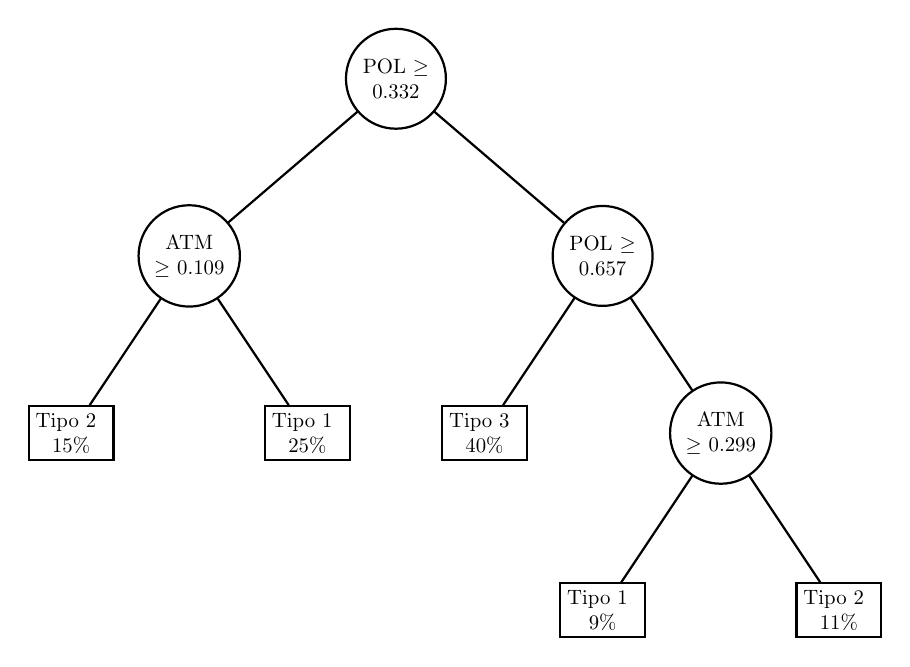
\begin{tikzpicture}[thick,scale=0.75, every node/.style={scale=0.75}]
\node [circle,draw,text width=1.2cm,align=center]{POL $\ge$ 0.332} [level distance=30mm,sibling distance=70mm]
child {node [circle,draw,text width=1.2cm,align=center] {ATM $\ge$ 0.109 } [level distance=30mm ,sibling distance=40mm]
child {node [rectangle,draw,text width=1.2cm,align=center] {Tipo 2\newline15\%}}
child {node [rectangle,draw,text width=1.2cm,align=center] {Tipo 1\newline25\%}}
}
child { node [circle,draw,text width=1.2cm,align=center]{ POL $\ge$ 0.657} [level distance=30mm ,sibling distance=40mm]
child {node [rectangle,draw,text width=1.2cm,align=center] {Tipo 3\newline40\%}}
child { node [circle,draw,text width=1.2cm,align=center]{ ATM $\ge$ 0.299 } [level distance=30mm ,sibling distance=40mm]
child {node [rectangle,draw,text width=1.2cm,align=center] {Tipo 1\newline9\%}}
child {node [rectangle,draw,text width=1.2cm,align=center] {Tipo 2\newline11\%}}
}
};
\end{tikzpicture}
\nota{Cada nó representa um atributo de um elemento da amostra. As folhas são consideradas a representação da classe a que uma observação pertence. Já o ramo é um conjunto de valores que reflete todas suas características e detalhes de um elemento}
\end{figure}


\begin{comment}

Seja \begin{math}p\end{math} os dados de entrada

Podemos representar de forma genérica o modelo da árvore por
\end{comment}


Suponha que exista \begin{math}M\end{math} partição que possa ser divida em regiões \begin{math}R_{1}, R_{2}, ..., R_{M} \end{math} e que seja possível modelar a resposta para cada região com a constante \begin{math}c_{m}\end{math}, 

\begin{equation}
f(x) = \sum_{m=1}^{M}c_{m}I( x \in R_{m} )
\end{equation}

Para a repartição dessas regiões, são definidos critérios para decidir de qual lado o dado irá ficar na árvore.


\subsubsection{Árvore de regressão}

No caso de uma regressão, utiliza-se como critério de minimização a soma do mínimos quadrados \begin{math}\sum{ (y_{i} - f(x_{i}))^{2}}\end{math}, temos que o melhor \begin{math}\hat c_{m}\end{math} é exatamente a média para \begin{math}y_{i}\end{math} na região \begin{math}R_{m}\end{math}:

\begin{equation}
\label{eq:media}
\hat c_{m} = m\acute edia(y_{i} | x_{i} \in R_{m})
\end{equation}

Para encontrar a melhor partição, é necessário recorrer a um algoritmo guloso.

Seja \begin{math}j\end{math} uma variável de reparticionamento, $s$ um ponto de divisão. É possível definir um par de semi planos 

\begin{equation}
R_{1}(j,s) = {X | X_{j}\leq s} \quad \textrm{e} \quad R_{2}(j,s) = {X | X_{j}\textgreater s})
\end{equation}

Resultando a busca pela de \begin{math}s\end{math} e \begin{math}j\end{math} que resolva

\begin{equation}
\min_{j,s} \left [ \min_{c_{1}} \sum_{x_{i} \in R_{1} (j,s)} (y_{i} - c_{1})^{2} + \min_{c_{1}} \sum_{x_{i} \in R_{2} (j,s)}(y_{i} - c_{2})^{2} \right ]
\end{equation} 


Mas como visto em \ref{eq:media}, temos que para qualquer $j$ e $s$, a minimização interna pode ser resolvida por:

\begin{equation}
\hat c_{1} = m\acute edia(y_{i} | x_{i} \in R_{1}(j,s)) \quad \textrm{e} \quad \hat c_{2} = m\acute edia(y_{i} | x_{i} \in R_{2}(j,s))
\end{equation} 

Este processo é repetido até que todas as regiões sejam descobertas.

\subsubsection{Árvore de classificação}

Para o caso de uma árvore de classificação, utiliza-se como critério de decisão a impureza de Gini\footnotemark \footnotetext{Impureza de Gini mede a frequencia de que um elemento selecionado aleatoriamente de um conjunto é marcado de forma errada} \begin{math}Gini(T) = 1 - \sum_{i=1}^{n}{ p_{i}^{2}}\end{math}. 

\subsection{\emph{Bagging}}

As árvores vistas anteriormente são modelos interessantes de classificação mas possuem um problema: o resultado gerado por elas em geral possuem uma acurácia muito baixa.



\begin{figure*}[t!]
    \centering
        \caption{Configurações da árvore de decisão sobre subconjuntos distintos}
    \begin{subfigure}[t]{0.5\textwidth}
        \centering
        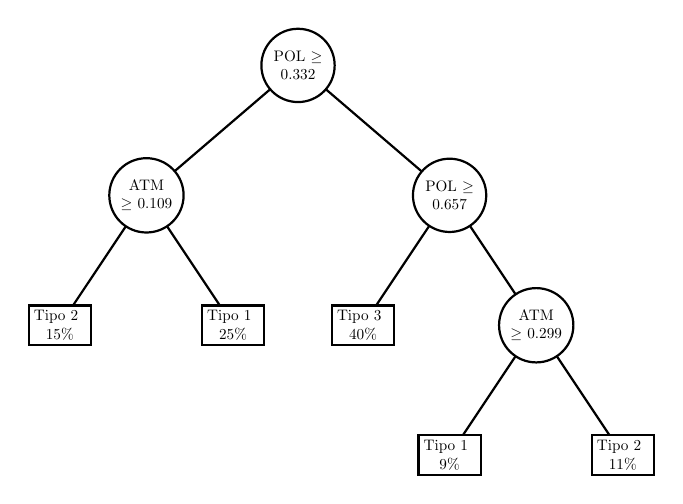
\begin{tikzpicture}[thick,scale=0.55, every node/.style={scale=0.55}]
\node [circle,draw,text width=1.2cm,align=center]{POL $\ge$ 0.332} [level distance=30mm,sibling distance=70mm]
child {node [circle,draw,text width=1.2cm,align=center] {ATM $\ge$ 0.109 } [level distance=30mm ,sibling distance=40mm]
child {node [rectangle,draw,text width=1.2cm,align=center] {Tipo 2\newline15\%}}
child {node [rectangle,draw,text width=1.2cm,align=center] {Tipo 1\newline25\%}}
}
child { node [circle,draw,text width=1.2cm,align=center]{ POL $\ge$ 0.657} [level distance=30mm ,sibling distance=40mm]
child {node [rectangle,draw,text width=1.2cm,align=center] {Tipo 3\newline40\%}}
child { node [circle,draw,text width=1.2cm,align=center]{ ATM $\ge$ 0.299 } [level distance=30mm ,sibling distance=40mm]
child {node [rectangle,draw,text width=1.2cm,align=center] {Tipo 1\newline9\%}}
child {node [rectangle,draw,text width=1.2cm,align=center] {Tipo 2\newline11\%}}
}
};
\end{tikzpicture}

        \caption{Configuração 1 da árvore de decisão}
    \end{subfigure}%
    ~ 
    \begin{subfigure}[t]{0.5\textwidth}
        \centering
        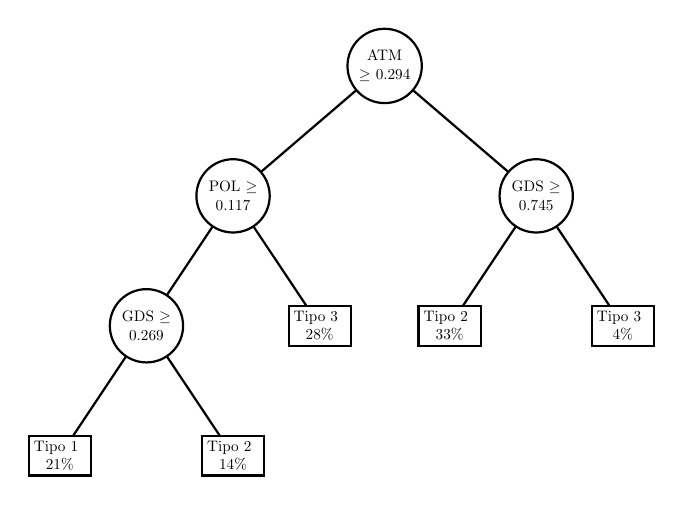
\begin{tikzpicture}[thick,scale=0.55, every node/.style={scale=0.55}]
\node [circle,draw,text width=1.2cm,align=center]{ATM $\ge$ 0.294} [level distance=30mm,sibling distance=70mm]
child { node [circle,draw,text width=1.2cm,align=center]{ POL $\ge$ 0.117 } [level distance=30mm ,sibling distance=40mm]
child { node [circle,draw,text width=1.2cm,align=center]{ GDS $\ge$ 0.269 } [level distance=30mm ,sibling distance=40mm]
child {node [rectangle,draw,text width=1.2cm,align=center] {Tipo 1\newline21\%}}
child {node [rectangle,draw,text width=1.2cm,align=center] {Tipo 2\newline14\%}}}
child {node [rectangle,draw,text width=1.2cm,align=center] {Tipo 3\newline28\%}}
}
child {node [circle,draw,text width=1.2cm,align=center] { GDS $\ge$ 0.745 } [level distance=30mm ,sibling distance=40mm]
child {node [rectangle,draw,text width=1.2cm,align=center] {Tipo 2\newline33\%}}
child {node [rectangle,draw,text width=1.2cm,align=center] {Tipo 3\newline4\%}}
};
\end{tikzpicture}
        \caption{Configuração 2 da árvore de decisão}
    \end{subfigure}


\end{figure*}



% \begin{figure*}[t!]
%     \centering
%     \begin{subfigure}[t]{0.5\textwidth}
%         \centering
%         \begin{tikzpicture}[thick,scale=0.55, every node/.style={scale=0.55}]
% \node [circle,draw,text width=1.2cm,align=center]{POL $\ge$ 0.332} [level distance=30mm,sibling distance=70mm]
% child {node [circle,draw,text width=1.2cm,align=center] {ATM $\ge$ 0.109 } [level distance=30mm ,sibling distance=40mm]
% child {node [rectangle,draw,text width=1.2cm,align=center] {Tipo 2\newline15\%}}
% child {node [rectangle,draw,text width=1.2cm,align=center] {Tipo 1\newline25\%}}
% }
% child { node [circle,draw,text width=1.2cm,align=center]{ POL $\ge$ 0.657} [level distance=30mm ,sibling distance=40mm]
% child {node [rectangle,draw,text width=1.2cm,align=center] {Tipo 3\newline40\%}}
% child { node [circle,draw,text width=1.2cm,align=center]{ ATM $\ge$ 0.299 } [level distance=30mm ,sibling distance=40mm]
% child {node [rectangle,draw,text width=1.2cm,align=center] {Tipo 1\newline9\%}}
% child {node [rectangle,draw,text width=1.2cm,align=center] {Tipo 2\newline11\%}}
% }
% };
% \end{tikzpicture}

%         \caption{Configuração 1 da árvore de decisão}
%     \end{subfigure}%
%     ~ 
%     \begin{subfigure}[t]{0.5\textwidth}
%         \centering
%         \begin{tikzpicture}[thick,scale=0.55, every node/.style={scale=0.55}]
% \node [circle,draw,text width=1.2cm,align=center]{ATM $\ge$ 0.294} [level distance=30mm,sibling distance=70mm]
% child { node [circle,draw,text width=1.2cm,align=center]{ POL $\ge$ 0.117 } [level distance=30mm ,sibling distance=40mm]
% child { node [circle,draw,text width=1.2cm,align=center]{ GDS $\ge$ 0.269 } [level distance=30mm ,sibling distance=40mm]
% child {node [rectangle,draw,text width=1.2cm,align=center] {Tipo 1\newline21\%}}
% child {node [rectangle,draw,text width=1.2cm,align=center] {Tipo 2\newline14\%}}}
% child {node [rectangle,draw,text width=1.2cm,align=center] {Tipo 3\newline28\%}}
% }
% child {node [circle,draw,text width=1.2cm,align=center] { GDS $\ge$ 0.745 } [level distance=30mm ,sibling distance=40mm]
% child {node [rectangle,draw,text width=1.2cm,align=center] {Tipo 2\newline33\%}}
% child {node [rectangle,draw,text width=1.2cm,align=center] {Tipo 3\newline4\%}}
% };
% \end{tikzpicture}
%         \caption{Configuração 2 da árvore de decisão}
%     \end{subfigure}
%     \\
%     \centering
%     \begin{subfigure}[t]{0.5\textwidth}
%         \centering
%         \begin{tikzpicture}[thick,scale=0.55, every node/.style={scale=0.55}]
% \node [circle,draw,text width=1.2cm,align=center]{POL $\ge$ 0.332} [level distance=30mm,sibling distance=70mm]
% child {node [circle,draw,text width=1.2cm,align=center] {ATM $\ge$ 0.109 } [level distance=30mm ,sibling distance=40mm]
% child {node [rectangle,draw,text width=1.2cm,align=center] {Tipo 2\newline15\%}}
% child {node [rectangle,draw,text width=1.2cm,align=center] {Tipo 1\newline25\%}}
% }
% child { node [circle,draw,text width=1.2cm,align=center]{ POL $\ge$ 0.657} [level distance=30mm ,sibling distance=40mm]
% child {node [rectangle,draw,text width=1.2cm,align=center] {Tipo 3\newline40\%}}
% child { node [circle,draw,text width=1.2cm,align=center]{ ATM $\ge$ 0.299 } [level distance=30mm ,sibling distance=40mm]
% child {node [rectangle,draw,text width=1.2cm,align=center] {Tipo 1\newline9\%}}
% child {node [rectangle,draw,text width=1.2cm,align=center] {Tipo 2\newline11\%}}
% }
% };
% \end{tikzpicture}

%         \caption{Configuração 1 da árvore de decisão}
%     \end{subfigure}%
%     ~ 
%     \begin{subfigure}[t]{0.5\textwidth}
%         \centering
%         \begin{tikzpicture}[thick,scale=0.55, every node/.style={scale=0.55}]
% \node [circle,draw,text width=1.2cm,align=center]{ATM $\ge$ 0.294} [level distance=30mm,sibling distance=70mm]
% child { node [circle,draw,text width=1.2cm,align=center]{ POL $\ge$ 0.117 } [level distance=30mm ,sibling distance=40mm]
% child { node [circle,draw,text width=1.2cm,align=center]{ GDS $\ge$ 0.269 } [level distance=30mm ,sibling distance=40mm]
% child {node [rectangle,draw,text width=1.2cm,align=center] {Tipo 1\newline21\%}}
% child {node [rectangle,draw,text width=1.2cm,align=center] {Tipo 2\newline14\%}}}
% child {node [rectangle,draw,text width=1.2cm,align=center] {Tipo 3\newline28\%}}
% }
% child {node [circle,draw,text width=1.2cm,align=center] { GDS $\ge$ 0.745 } [level distance=30mm ,sibling distance=40mm]
% child {node [rectangle,draw,text width=1.2cm,align=center] {Tipo 2\newline33\%}}
% child {node [rectangle,draw,text width=1.2cm,align=center] {Tipo 3\newline4\%}}
% };
% \end{tikzpicture}
%         \caption{Configuração 2 da árvore de decisão}
%     \end{subfigure}
%     \caption{Configurações da árvore de decisão sobre subconjuntos distintos}
% \end{figure*}

Dessa forma, uma solução para contornar esse problema foi a adaptação de uma técnica chamada \emph{bootstraping aggregating}, que constrói uma árvore de classificação repetidamente usando amostras aleatórias do conjunto de dados. Por fim, o modelo final é recalculado.
